%% Template for ENG 401 reports
%% by Robin Turner
%% Adapted from the IEEE peer review template

%
% note that the "draftcls" or "draftclsnofoot", not "draft", option
% should be used if it is desired that the figures are to be displayed in
% draft mode.

\documentclass{article}
\usepackage{url} % Provides better formatting of URLs.
\usepackage[utf8]{inputenc} % Allows Spanish characters.
\usepackage[spanish]{babel}
\usepackage{amssymb}
\usepackage{booktabs} % Allows the use of \toprule, \midrule and \bottomrule in tables for horizontal lines
\usepackage{float}
\usepackage{pdfpages}
\usepackage{graphicx}
\usepackage{booktabs}
\usepackage{fancyhdr}
\usepackage{eurosym}
\usepackage{calendar}



\hyphenation{op-tical net-works semi-conduc-tor} % Corrects some bad hyphenation 



\begin{document}
%\begin{titlepage}
% paper title
% can use linebreaks \\ within to get better formatting as desired
\title{
\includegraphics[scale=0.65]{logoDefinitivo1.png} \\ \textbf{Proyecto UPBEAT} \\ \textbf{Grupo 03. Barbara Liskov}\\Plan de gestión, análisis y memoria del proyecto \vspace{0.1cm} \\}

% author names and affiliations

\author{Alejandro Ruiz Sumelzo\\
Alejandro Piedrafita Barrantes\\
Álvaro Santamaría De la Fuente\\
Fernando Navarro Zarralanga\\
José Félix Yagüe Royo\\
Víctor Pérez Sanmartín\\
Sergio Torres Castillo \vspace{0.25cm}
\\\\

\includegraphics[scale=0.5]{logoUZ.png}\\
}
\date{24 de febrero de 2020}

% make the title area
\maketitle
\newpage
\section*{Introducción}
El proyecto \textit{Upbeat} consiste en el desarrollo e implementación de un reproductor de música en streaming.
\hfill \break
La aplicación está diseñada para todo tipo de público, incluidos artistas. Permitirá a los usuarios escuchar música, crear listas de reproducción o seguir a otros usuarios entre otras funcionalidades.
\hfill \break
De manera similar, los artistas tendrán las mismas características que cualquier usuario además de poder subir canciones y/o álbumes.
\hfill \break
Añadirá aspecto de la 'red social', tales como seguir a otros usuarios o sus playlist creadas.
\hfill \break
Se permitirá usar la aplicación de tres maneras diferentes: web, Android e iOS.
Usará también un sistema de sincronización, permitiendo que el usuario retome cualquier canción donde la había dejado, en todos los dispositivos.

\newpage
\tableofcontents % si estas líneas se comentan, se eliminan los índices
%\listoffigures
%\listoftables
\addtocontents{toc}{\hfill \textbf{Página} \par}
\newpage
\pagestyle{fancy}
\lhead{\begin{picture}(0,0) \put(0,0){\includegraphics[width=40mm]{logoEina.png}} \end{picture}}
\rhead{\begin{picture}(0,0) \put(-100.7,0){
\includegraphics[width=35mm]{logoDefinitivo3.png}} \end{picture}}
\section{Organización del proyecto}
\begin{table}[H]
	\hspace*{-3.7cm}
	\centering
	\begin{tabular}{|l|l|l|}
		\hline
		\multicolumn{1}{|c|}{\textbf{Integrante}} & \multicolumn{1}{c|}{\textbf{Puesto}} & \multicolumn{1}{c|}{\textbf{Responsabilidades}}\\ \hline
		Alejandro Ruiz Sumelzo                    & \begin{tabular}[c]{@{}l@{}}Director del proyecto.\\ Coordinador y desarrollador del grupo de back-end.\\ Encargado de la documentación del análisis y diseño\\ del sistema.\end{tabular} & \begin{tabular}[c]{@{}l@{}}Responsable de redactar algunas actas\\ en reuniones con el profesor.\\ Control de la distribución de trabajo\\ (elaboración de calendario) y \\ revisión de esfuerzos.\\ Desarrollador de modelos, repositorios y \\controladores de la API.\\ Encargado del despliegue del back end \\sobre el servidor.\end{tabular} \\ \hline
		\begin{tabular}[c]{@{}c@{}}Alejandro\\ Piedrafita Barrantes\end{tabular}
		&                                                                       Desarrollador de apoyo para el grupo de back-end                                                                                                                 &  
		\begin{tabular}[c]{@{}l@{}}Realización de tareas de gestión\\  (edición de memoria y otros documentos).\\ Desarrollador de modelos, repositorios y \\ controladores de la API. \\ Diseño del sistema mediante diagramas.\end{tabular}\\ \hline
		\begin{tabular}[c]{@{}c@{}}Víctor\\ Pérez Sanmartín\end{tabular}
		&                                                                       Desarrollador de apoyo para el grupo de back-end                                                                                                                 &  
		\begin{tabular}[c]{@{}l@{}}
		Responsable de redactar algunas actas\\ en reuniones con el profesor.\\
		Realización de tareas de gestión\\  (edición de memoria y otros documentos).\\ Desarrollador de modelos, repositorios y \\ controladores de la API. \\ Encargado del diseño e implementación\\ de la base de datos.\end{tabular}\\ \hline
		\begin{tabular}[c]{@{}c@{}}Álvaro Santamaría\\ de la Fuente\end{tabular}
		& \begin{tabular}[c]{@{}l@{}}  Desarrollador del grupo de front-end móvil.\\ Encargado de la gestión de la parte front móvil \\ del proyecto.\end{tabular}     &  
		\begin{tabular}[c]{@{}l@{}}
		Realización de tareas de gestión\\ (edición de memoria y otros documentos).\\
		Desarrollo e implementación del front-end \\de la aplicación móvil.\\
		Implementar la lógica de la aplicación de\\ Android e iOS.\\
		Encargado de unificar las partes \\de la aplicación móvil y llevar a cabo \\ el despliegue en Android e iOS.
		\end{tabular}\\ \hline
		\begin{tabular}[c]{@{}c@{}}José Félix \\ Yagüe Royo\end{tabular}
		&                                                                       Coordinador y desarrollador de apoyo para el grupo de front-end                                                                                                                 &  
		\begin{tabular}[c]{@{}l@{}}Realización de tareas de gestión\\ (edición de memoria y otros documentos).\\
		Desarrollo e implementación del front end \\de la aplicación móvil.\\
		Encargado de la conexión con el API REST. \\
		Control de la distribución de trabajo y \\ coordinación dentro del grupo \\ front-end de móvil.\\\end{tabular}\\ \hline
	\end{tabular}
\end{table}

\begin{table}[H]
	\hspace*{-3.7cm}
	\centering
	\begin{tabular}{|l|l|l|}
		\hline
		\multicolumn{1}{|c|}{\textbf{Integrante}} & \multicolumn{1}{c|}{\textbf{Puesto}} & \multicolumn{1}{c|}{\textbf{Responsabilidades}}\\ \hline
		\begin{tabular}[c]{@{}c@{}}Fernando\\ Navarro Zarralanga\end{tabular}           
		& 
		\begin{tabular}[c]{@{}l@{}}Coordinador y desarrollador del grupo de \\ front-end web.\\ Encargado de la gestión de la parte front web \\ del proyecto.\end{tabular} & \begin{tabular}[c]{@{}l@{}}Realización de tareas de gestión\\ (edición de memoria y otros documentos).\\ Diseñar pantallas de la aplicación de la web.\\
		Implementar la lógica de la \\ aplicación web.\\ 
		Encargado de llevar a cabo el despliegue \\de la web.
		\end{tabular} \\ \hline
		\begin{tabular}[c]{@{}c@{}}Sergio\\ Torres Castillo\end{tabular}
		&                                                                       Desarrollador de apoyo para el grupo de front-end                                                                                                                 &  
		\begin{tabular}[c]{@{}l@{}}
			Realización de tareas de gestión\\ (edición de memoria y otros documentos).\\
			Diseñar pantallas de la aplicación de la web.\\ Implementar parte de la lógica de la \\aplicación web.\end{tabular}\\ \hline
	\end{tabular}
\end{table}
\newpage
\section{Plan de gestión del proyecto}

\subsection{Procesos}

\subsubsection{Procesos de inicio del proyecto}

\subsubsection{Procesos de ejecución y control del proyecto}
Las comunicaciones internas se llevarán a cabo mediante un grupo de WhatsApp estimado para ello, para cualquier otra duda o comunicación entre componentes del equipo se hará de forma individual. La resolución de tareas será totalmente independiente y completa en el entorno de GitHub.
\hfill \break
Los responsables de realizar la puesta en marcha serán los encargados de la parte front-end y de la parte back-end. La creación de copias de seguridad y semejantes se realizarían de manera automática gracias a GitHub. 
\hfill \break
El repositorio que se creará con todos los archivos referentes al proyecto se encontrará en GitHub, para que todos los integrantes del proyecto puedan acceder fácilmente a los archivos. Además, se usará el \textit{Issue Tracker} de GitHub para la gestión de incidencias; el director del mismo se encargará de crear las incidencias principales, y cada uno de los encargados de cada parte las completarán en cada uno de sus ámbitos. 
\hfill \break
El proyecto estará dividido en varios repositorios: uno específico para front-end, otro para back-end, y la memoria. Para conseguir que no se modifique el mismo fichero por dos personas al mismo tiempo y evitar problemas, cada equipo tendrá más sub-ramas de desarrollo, por ejemplo, una para cada miembro del equipo, que serán actualizadas con cambios no siempre funcionales y cuando sean más estables se volcarán a la rama de desarrollo principal. 
\hfill \break
En la rama principal de cada uno de los repositorios, sólo podrá haber una versión funcional del sistema, que antes de ser subida será sometida a diferentes test automáticos, entre los que se incluirán test para comprobar la estabilidad del sistema (pruebas de sobrecarga) y test que revisarán las acciones disponibles para comprobar los requisitos que se han resuelto, además de ser testeado por varios miembros del equipo. 
\hfill \break
Para que lo desarrollado en cada uno de estos repositorios pase al repositorio funcional, cada líder de las respectivas partes revisará el código actualizado y si todo está correcto se considerará válido. 
\hfill \break
Todas las semanas habrá una serie de tareas asociadas mediante el \textit{Issue Tracker}. Al final de cada semana, el responsable de cada parte del proyecto revisa las tareas que se han realizado esa semana y se realiza un seguimiento de las mismas: si hay tareas que no se han cumplido, se asigna automáticamente para la siguiente semana, siendo estas tareas las primeras que se deberán hacer.  
\hfill \break
Además, cada semana el responsable de cada una de las partes revisará cuántas tareas se han realizado para la siguiente iteración, controlando si han sido completadas o no y cuánto tiempo de retraso acumula respecto a la planificación original.  Tras esta revisión, este responsable asignará las tareas de la semana a todos los miembros del equipo que puedan trabajar esa semana. 
\hfill \break
Durante el desarrollo del proyecto puede haber problemas y disputas entre los miembros del equipo. Para tratar de resolverlos los coordinadores serán los primeros en mediar entre los miembros en disputa y, si hay alguna razón que haga imposible esta mediación, será el resto del equipo quien deberá votar en consecuencia. 
\hfill \break
Todos los componentes del equipo son capaces de modificar los ficheros de los repositorios, excepto en el de las versiones, el cual solo podrán subir archivos y modificarlos los líderes del front-end y el back-end.

\subsubsection{Procesos técnicos}
Para el desarrollo del software de la parte del Front-end de la aplicación móvil se va a utilizar el entorno de Android Studio haciendo uso de su integración con \textit{git} para facilitar el control de versiones y así, gestionar de forma uniforme entre los dos integrantes del grupo, el repositorio \textit{"}Flutter\textit{"} en el que se irá desarrollando el software correspondiente a la aplicación móvil. Para las pruebas en el dispositivo de iOS se utilizará el entorno de VSCode.\\\\
Para el proceso de prueba de funcionalidades de la aplicación móvil se seguirá el siguiente guión:
	\begin{itemize}
		\item Primero el desarrollador se asegurará de tener la última versión del repositorio \textit{"}Flutter\textit{"}, efectuando un pull de la rama que desea testear.
		
		\item A continuación se abre el entorno de desarrollo (VSCode en caso de que se vaya a probar la aplicación en iOS o Android Studio en el caso de un dispositivo Android) y se procede a buildear el código de la app. En caso de encontrar errores se notificarán al encargado de haber realizado esa parte del código.
		
		\item Se ejecuta la aplicación libre de errores de compilación en el dispositivo deseado (iOS o Android)
		
		\item Posteriormente se realiza la prueba de la nueva funcionalidad implementada, comprobando que no se dan situaciones de error ni resultados inesperados.
		
		\item Si las pruebas realizados han sido satisfactorias, se informará al coordinador del grupo de front-end móvil y realizará un merge de esa rama con la rama máster.
	\end{itemize}
\newpage
\subsection{Planes}

\subsubsection{Plan de gestión de configuraciones}
La convención de nombres utilizadas para nombrar los distintos archivos sería la siguiente: 
\begin{figure}[H]
	\centering{
		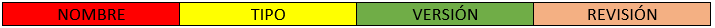
\includegraphics[scale=0.55]{conf1.png}}
\end{figure}
Las versiones solo se modificarán cada vez que se produzcan cambios suficientemente importantes, como por ejemplo la implementación de una nueva funcionalidad. 
Cada vez que se cree una nueva versión, pero sus cambios sean menores, como resolución de errores, se modificará su número de revisión, pero no de versión. 
Se crearán ficheros de documentación que permita ir recopilando toda la información referente a los cambios.
Además, en los ficheros de documentación en los que se expliquen las diversas funcionalidades que tiene la aplicación y que errores se han ido resolviendo, cuando estos sean de una nueva versión o revisión solo se ofrecerá la información sobre los cambios que existan entre esta y la versión o revisión anterior, pero siempre que se cambie la versión se documentarán los cambios respecto a la primera revisión de la versión anterior (p.ej. La versión 2.1 solo contendrá las novedades respecto a la versión 2.0, pero la versión 3.0 contendrá todos los cambios que hayan sucedido desde la versión 2.0 aunque la mayoría se hayan documentado ya en las revisiones). 

\newpage
\subsubsection{Plan de construcción y despliegue del software}

\subsubsection{Plan de aseguramiento de la calidad}

\newpage

\subsubsection{Calendario del proyecto y división del trabajo}
En la primera iteración del proceso de diseño nos centraremos en desarrollar las funcionalidades principales del sistema, mientras que en la segunda iteración se corregirán todos los errores encontrados en la primera, se implementarán las funcionalidades secundarias y se afinara el diseño de la página web y de las aplicaciones móviles para que sean más agradables al usuario. 
\hfill \break
Para la primera iteración, se planea permitir la creación, edición y borrado de clientes con sus credenciales básicos: nombre de usuario, nombre real, correo, contraseña. Unido a esto, comprobar si las entidades Artista y Usuario se crean y borrar correctamente.  También se permitirá la subida de canciones por parte de los artistas; estas canciones serán visibles en la aplicación y podrán ser reproducidas (al igual que los podcasts). Los álbumes estarán disponibles con su descripción y podrán ser consultados, reproduciendo cada una de sus canciones.
\hfill \break
Para la segunda iteración se finalizarán los requisitos que, por falta de tiempo, no pudieron ser completados en la primera y se añadirán funcionalidades al sistema. Estas funcionalidades son: añadir canciones a la lista de reproducción de un usuario, permitir información adicional en los perfiles de usuario (como puede ser una foto de perfil, una descripción, etc.), además de poder seguirse entre dos usuarios. Se permitirá la búsqueda y filtrado de determinadas canciones y/o álbumes por unos determinados parámetros, al igual que utilizar un ecualizador en la aplicación web con el uso de \textit{banners}.

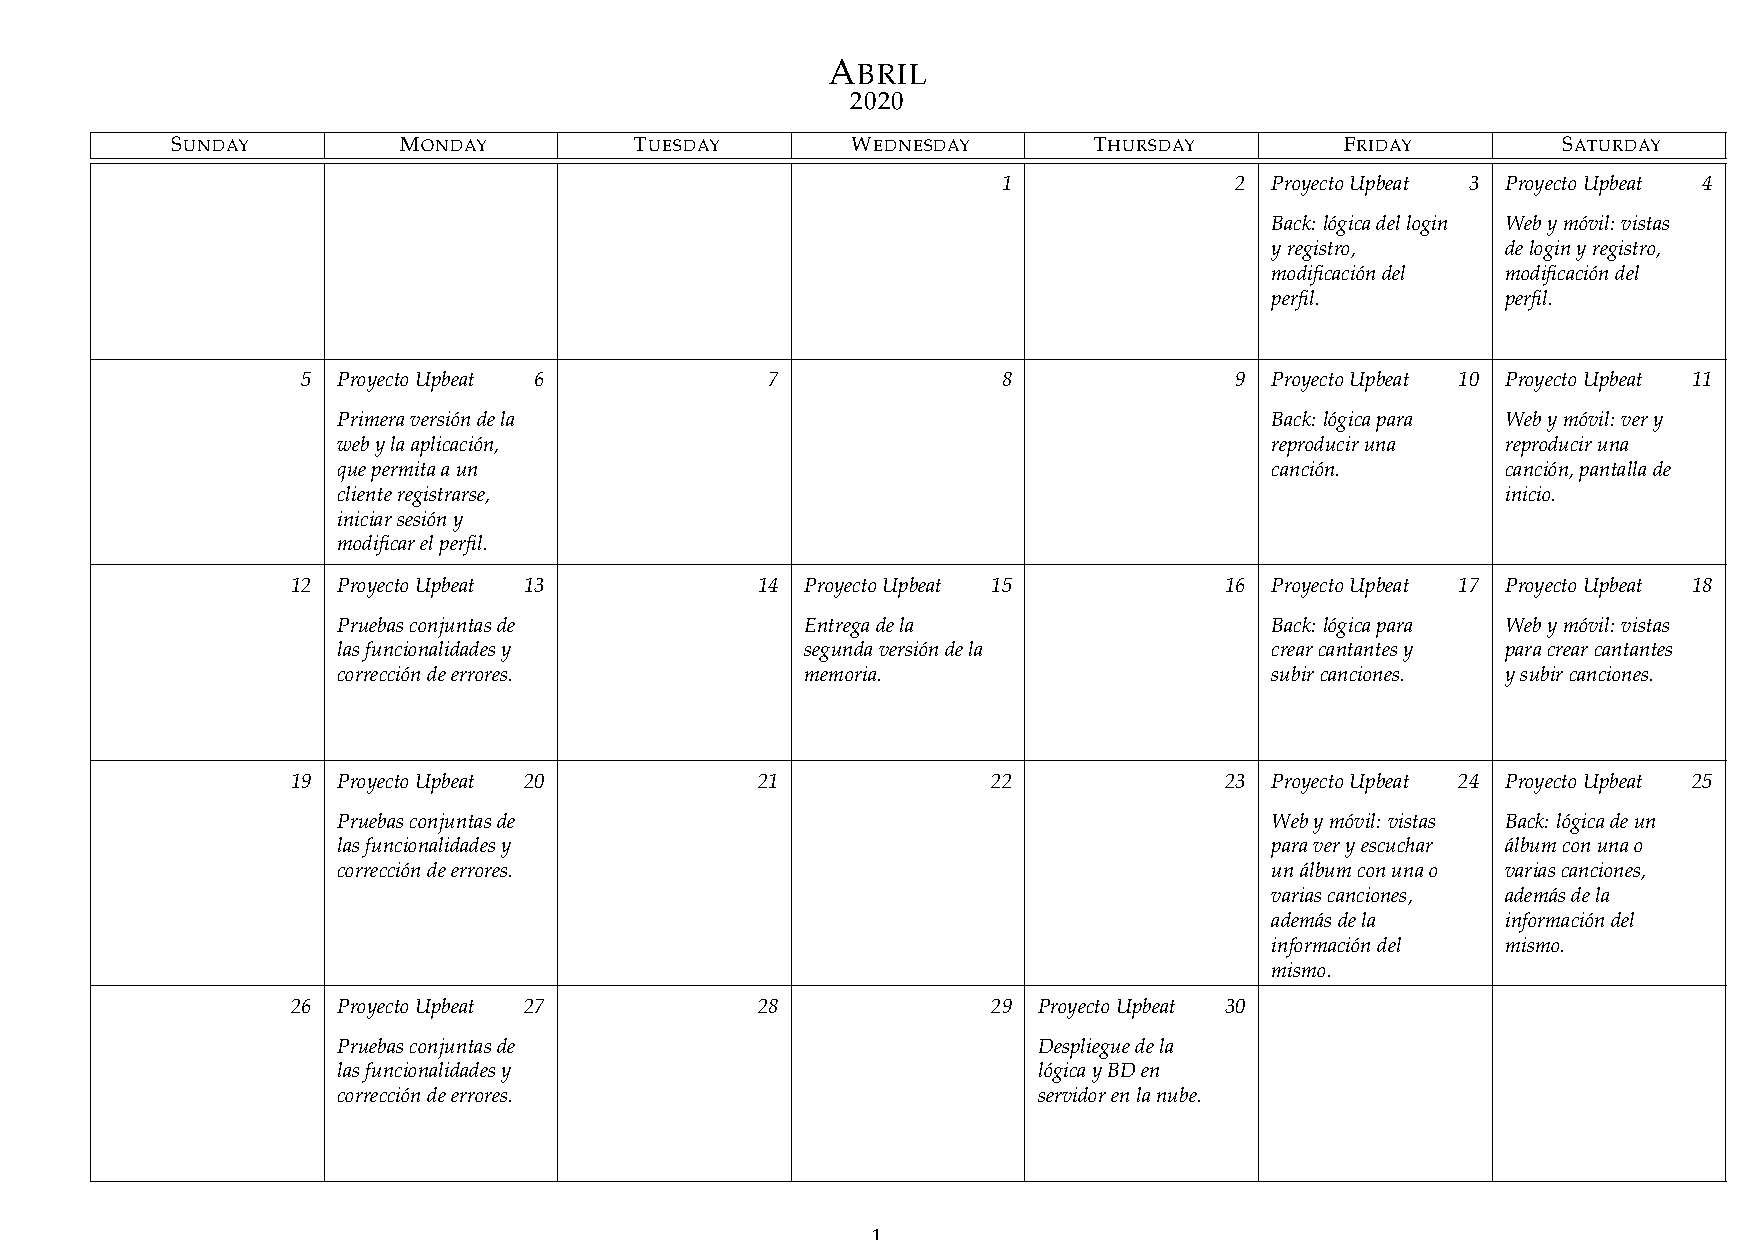
\includepdf[pages=1-2]{calendar.pdf}
\newpage
\section{Análisis y diseño del sistema}

\subsection{Análisis de requisitos}
Se exponen los siguientes requisitos funcionales de la aplicación:
\begin{table}[H]
	\begin{tabular}{p{4cm} p{10cm}}
		\hline
		\hline 
		\textbf{Requisito funcional}
		\vspace{0.5mm} & \textbf{Descripción} \\ 
		\hline
		\hline
		RF1
		& El sistema permite la existencia de clientes. \\ 
		\hline 
		RF2
		& Los clientes podrán ser usuarios normales o artistas. \\ 
		\hline
		RF3
		& Los clientes se registrarán mediante usuario y contraseña. \\ 
		\hline
		RF4
		& Un usuario es un cliente registrado que puede acceder a las funciones de la aplicación como escuchar canciones/podcasts, crear y seguir listas de reproducción, seguir a otros usuarios, escuchar álbumes y ver las canciones subidas por los artistas. \\ 
		\hline
		RF5
		& Un artista es un cliente registrado que puede realizar las mismas funciones que un usuario, además de crear álbumes y subir canciones. Crear un álbum consiste en la creación de un grupo de canciones que pertenecen al mismo artista. \\ 
		\hline
		RF6
		& Un cliente se compone de un nombre único, nombre personal y apellidos, un correo electrónico, una contraseña para acceder a la aplicación, una foto de perfil y las redes sociales que posee (si quiere añadirlas de forma opcional). \\ 
		\hline
		RF7
		& El sistema permite que los clientes modifiquen los datos de su perfil, es decir, su nombre, correo, contraseña, foto de perfil e información de las redes sociales. \\ 
		\hline
		RF8
		& Los clientes accederán a la aplicación mediante una aplicación móvil o una aplicación web. \\ 
		\hline
		RF9
		& El sistema permite reproducir y pausar una canción y/o podcasts. También permite saltar a la siguiente (si la hubiera), retroceder a la anterior, y elegir un bucle de la misma o reproducir aleatoriamente varias canciones y/o podcasts. \\ 
		\hline
		RF10
		& Una canción se compone de un título, un audio, artista/s que la han creado, género de la canción, país de la canción y veces que ha sido reproducida. \\ 
		\hline
		RF11
		& Una lista de reproducción es una lista de canciones generadas por un cliente. \\ 
		\hline
		RF12
		& El sistema permite que un cliente cree y borren listas de reproducción creados por ellos mismos, las cuales serán públicas. \\ 
		\hline
		RF13
		& El sistema permite que los clientes añadan canciones a las listas de reproducción creadas por ellos mismos. \\ 
		\hline
		RF14
		& El sistema permite que los clientes sigan listas de reproducción creadas por otros usuarios. \\ 
		\hline
		RF15
		& El sistema permite que solo los artistas puedan subir canciones. \\ 
		\hline
		RF16
		& El sistema permite buscar una determinada canción por nombre o género, además de un artista por nombre. \\ 
		\hline
	\end{tabular}
\end{table}
\break
\begin{table}[H]
	\begin{tabular}{p{4cm} p{10cm}}
		\hline
		\hline 
		\textbf{Requisito funcional}
		\vspace{0.5mm} & \textbf{Descripción} \\ 
		\hline
		\hline
		RF17
		& Las búsquedas por palabras clave deberán al menos contener una palabra, de mínimo cuatro caracteres. \\ 
		\hline 
		RF18
		& El sistema permite ver las canciones más populares de un país. \\ 
		\hline 
		RF19
		& El sistema permite ver las canciones más populares de un artista. \\ 
		\hline
		RF20
		& El sistema permitirá usar un equalizador al escuchar las canciones. \\ 
		\hline
		RF21
		& El sistema permitirá el uso de \textit{banners} para ofrecer publicidad. \\ 
		\hline
	\end{tabular}
\end{table}
Se exponen los siguientes requisitos no funcionales de la aplicación:

\begin{table}[H]
	\begin{tabular}{p{4cm} p{10cm}}
		\hline
		\hline 
		\textbf{Requisito no funcional} & \textbf{Descripción} \\ 
		\hline
		\hline
		RNF1 
		&  El sistema permitirá ser utilizar un diseño modular, un lenguaje fácil de entender, usar y mantener.\\ 
		\hline
		RNF2
		&  La seguridad será fundamental a la hora de garantizar la confidencialidad y autentificación de las canciones, así como para cumplir determinados aspectos de la LOPD y los derechos de los cantautores.\\ 
		\hline
		RNF3
		&  El cliente tendrá el desarrollo móvil en formato Android e iOS.\\ 
		\hline
		RNF4
		& El sistema permite almacenar canciones y podcasts en formato \textit{.mp3}, \textit{.WAV} y \textit{.OGG}. \\
	\end{tabular}
\end{table}
\newpage

\subsection{Diseño del sistema}

\end{document}


